% \begin{wrapfigure}{l}{0.4\textwidth}                   
\begin{center}
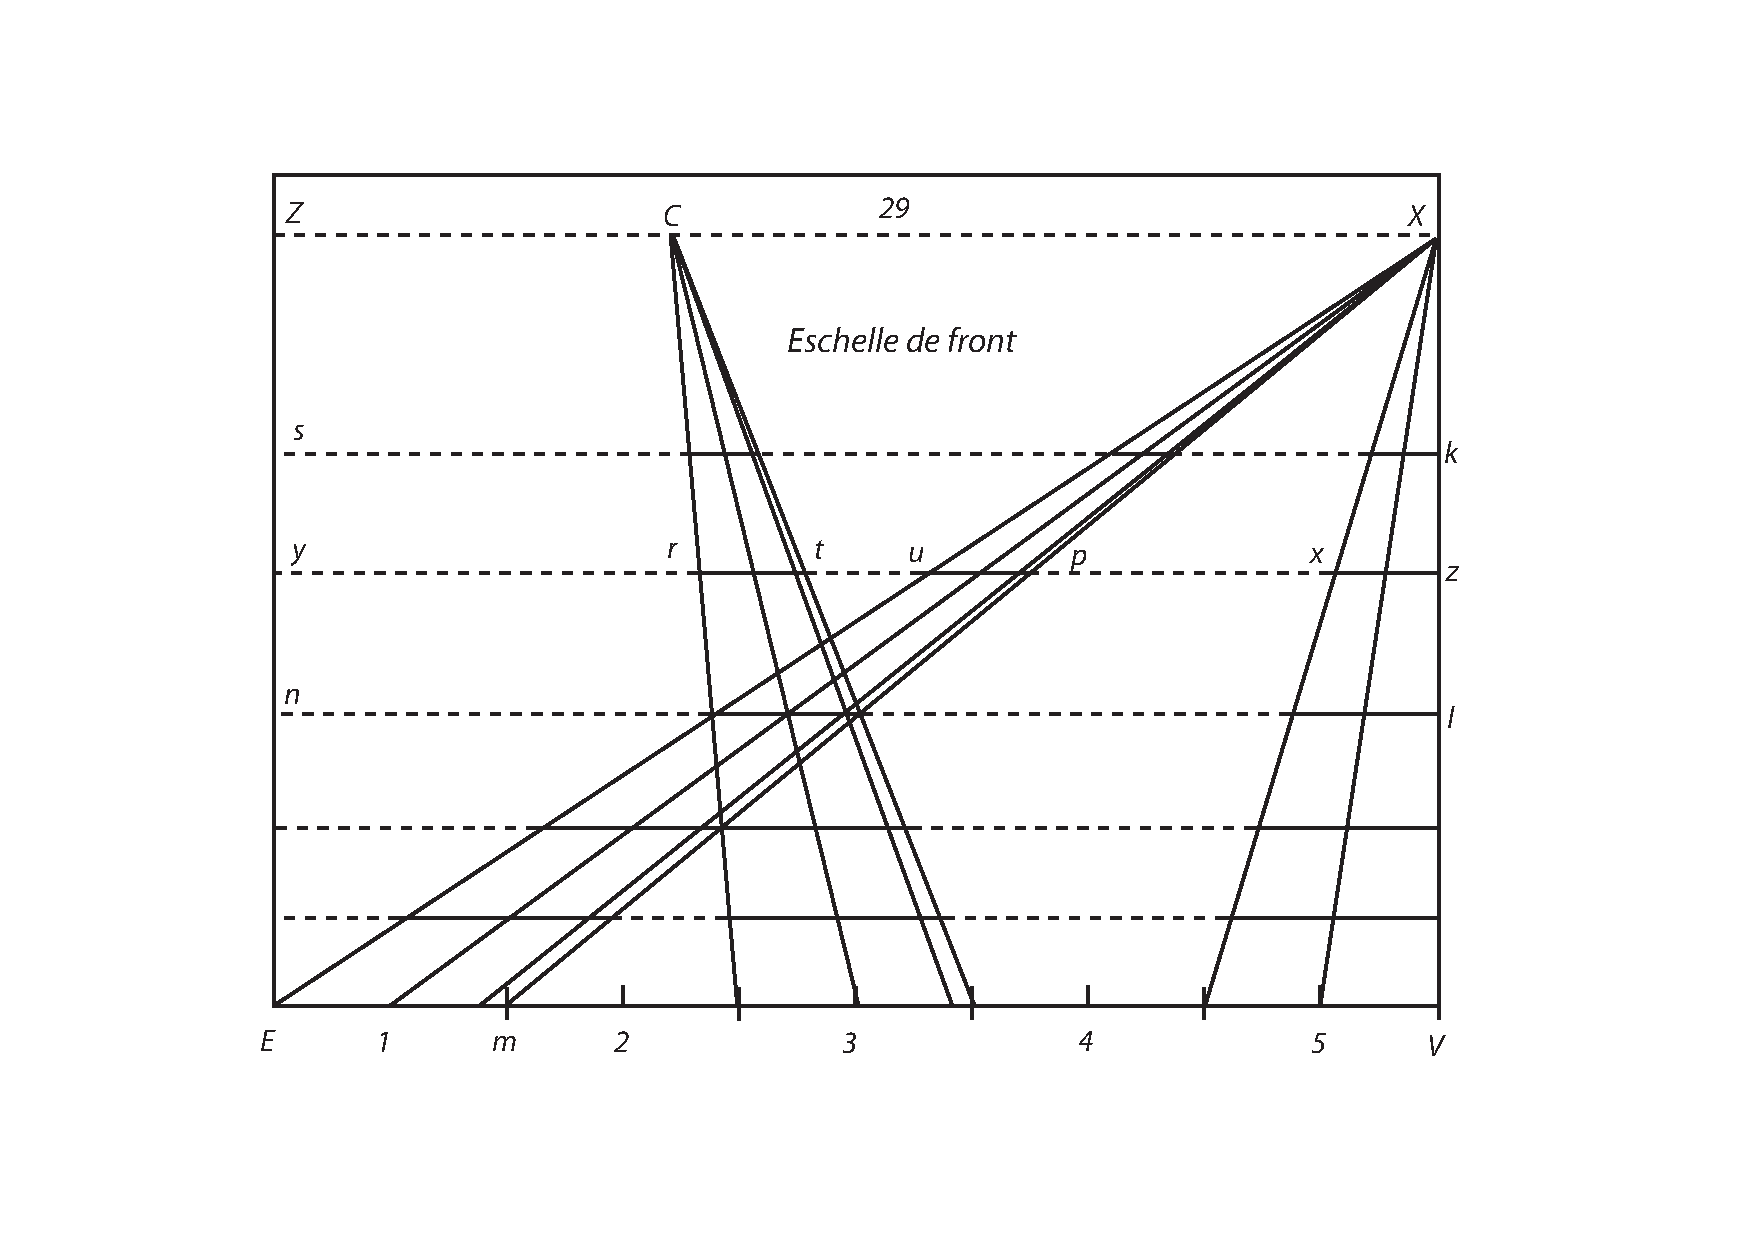
\includegraphics[width=1\textwidth]{images/T29-Desargues_87_a}
\\\textit{[Fig. 12a]}
\footnote{\textit{\"{U}ber der Strecke tu}: \textit{rt} \'{e}gal \`{a} \textit{up} ou \`{a} \textit{xz}}
\end{center}
\begin{center}
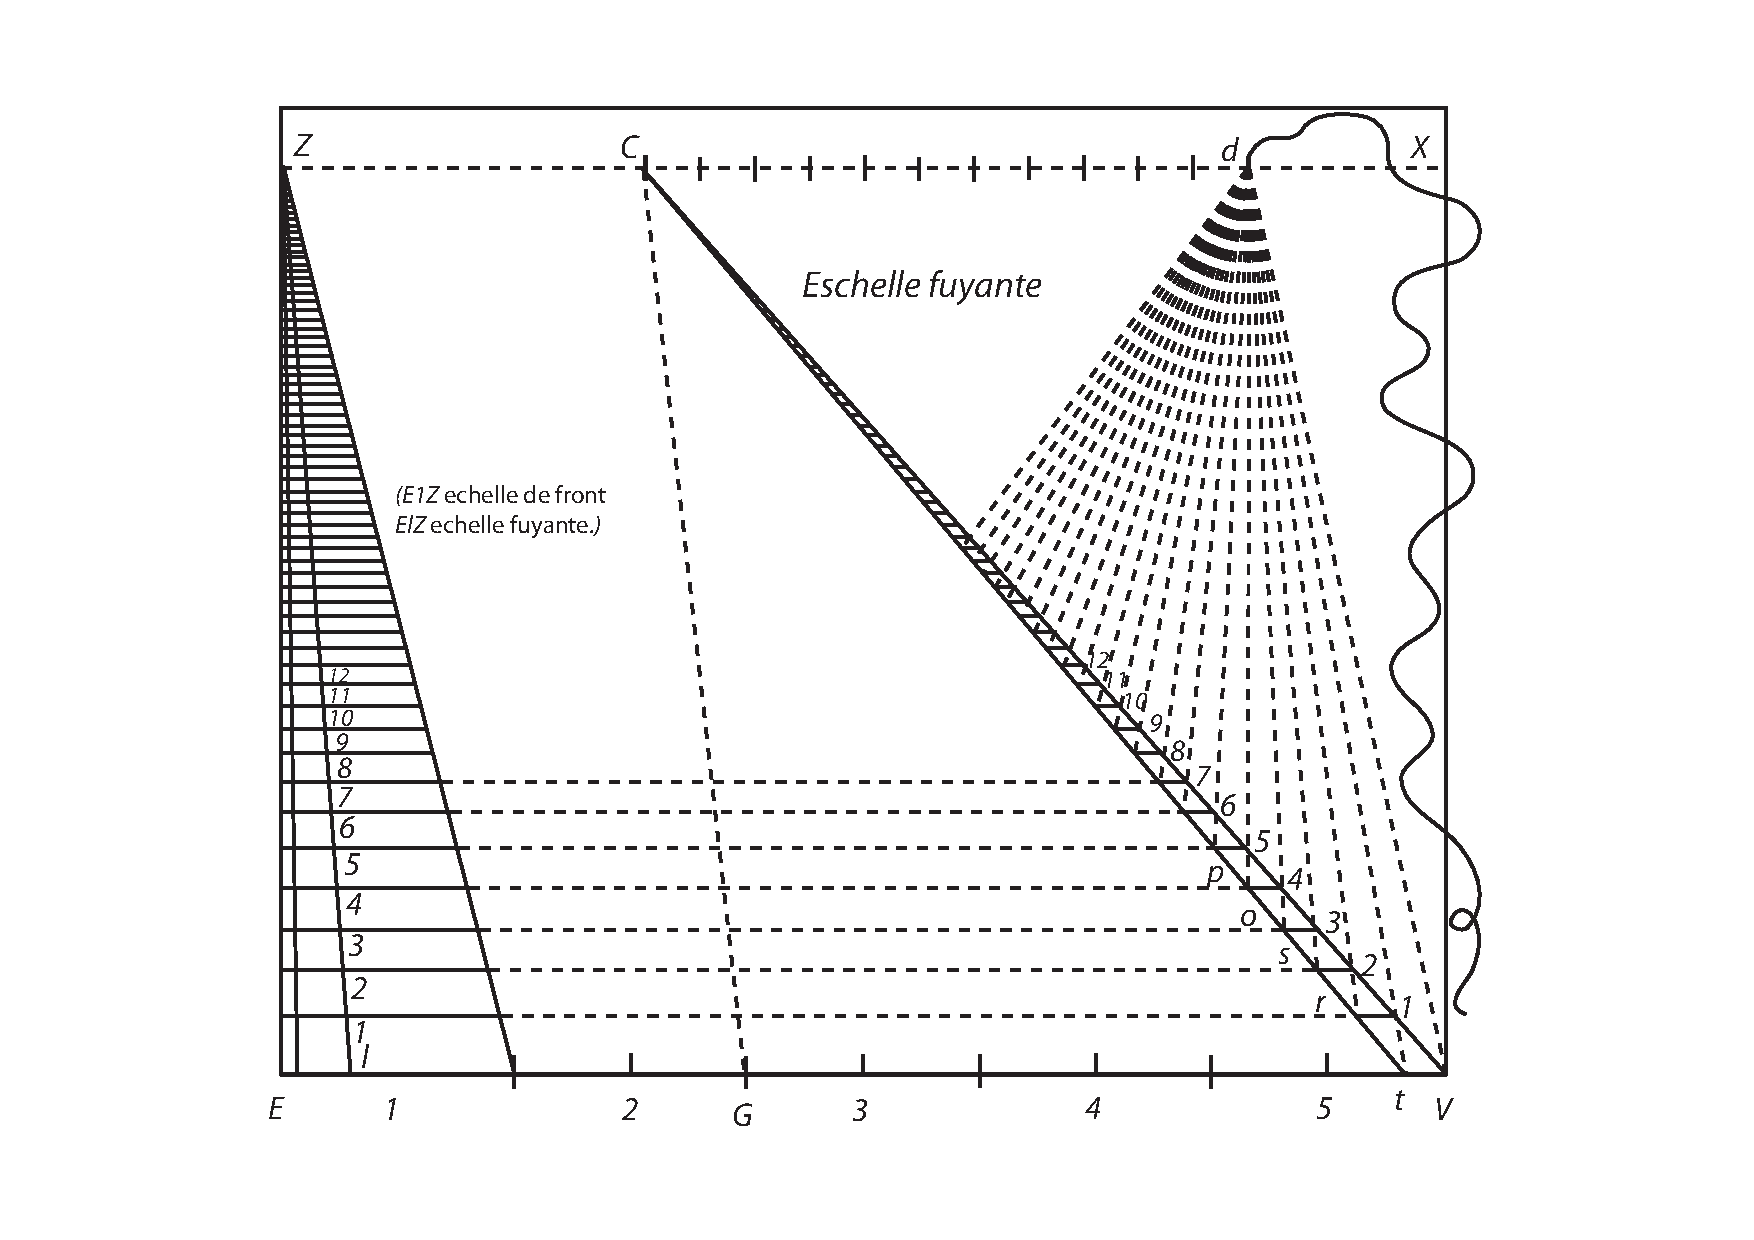
\includegraphics[width=1\textwidth]{images/T29-Desargues_87_b}
\\\textit{[Fig. 12b]}
\footnote{\textit{Links unter der Geraden ZX}: \textit{cd} \`{a} \textit{Vt} ou \`{a} \textit{dh} comme la distance de la station \`{a} la conduite de front est \`{a} un pied \textit{E1}. \\ \textit{Rechts unter der Geraden }\textit{ZX}: \textit{dh} \'{e}gal \`{a} \textit{Vt} \\ \textit{Oben links neben der Geraden CV}: \protect\begin{tabular}{c} dp\\do\protect\end{tabular} coupe \textit{CV} en \protect\begin{tabular}{c} 5\\4\protect\end{tabular}\rule[-4mm]{0mm}{10mm}  \\ \textit{Im unteren Teil der Abbildung in der Mitte links neben der Geraden CV}: \textit{E1Z} echelle de front\protect\index{Sachverzeichnis}{\'{e}chelle!de front} \textit{ElZ} echelle fuyante\protect\index{Sachverzeichnis}{\'{e}chelle!fuyante}.} 
\end{center}